% practico.tex
\section{Parte Práctica}

Para resolver este trabajo desarrollamos dos componentes: un módulo de kernel (CDD) que genera y expone dos señales periódicas, y una aplicación de usuario que las lee, grafica y permite cambiar de una a otra.

En el espacio núcleo:
\begin{itemize}
  \item Se creó un \texttt{Makefile} que invoca la construcción de un módulo de caracteres (\texttt{modulo\_signals.ko}) usando la infraestructura estándar de compilación del kernel.
  \item El driver registra un dispositivo \texttt{/dev/mis\_senales} y emplea un \emph{timer} del kernel para actualizar dos señales cada segundo:
    \begin{enumerate}
      \item Una señal contadora cíclica (0–99).
      \item Una onda triangular (0–100).
    \end{enumerate}
  \item A través de las operaciones \texttt{read} y \texttt{write} del driver, el usuario elige cuál de las dos señales sensar y lee su valor actual.
\end{itemize}

En espacio de usuario:
\begin{itemize}
  \item Se escribió un script en Python que abre \texttt{/dev/mis\_senales}, envía \texttt{'0'} o \texttt{'1'} para seleccionar la señal y, cada segundo, lee el valor devuelto.
  \item Utilizando \texttt{matplotlib.animation}, el programa dibuja en tiempo real el valor de la señal contra el tiempo, etiqueta ejes y título según la señal activa, y reinicia el gráfico cuando se cambia de señal.
  \item Este enfoque separa claramente la lógica de sensado (kernel) de la de presentación y ajuste de escala (usuario).
\end{itemize}

Para el desarrollo se recomendó emplear una Raspberry Pi, aprovechando su soporte nativo de módulos del kernel y su facilidad para conectar sensores o dispositivos externos.

\subsection{Visualización de la Señal}

\begin{figure}[H]
  \centering
  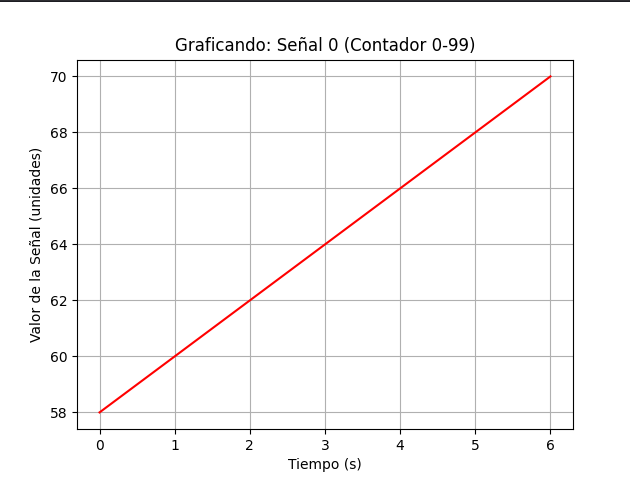
\includegraphics[width=0.8\textwidth]{img/graphic.png}
  \caption{Evolución de la Señal 0 (contador cíclico).}
  \label{fig:signal0}
\end{figure}

La Figura~\ref{fig:signal0} muestra cómo la Señal 0 avanza de 0 a 99 en pasos de 2 unidades por segundo. 

\begin{figure}[H]
  \centering
  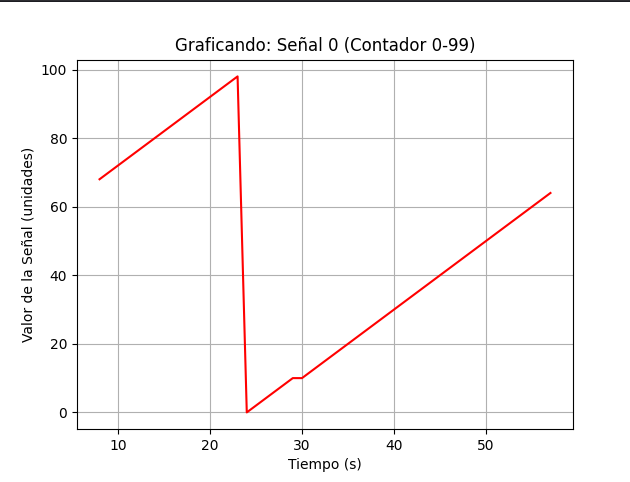
\includegraphics[width=0.8\textwidth]{img/graphic2.png}
  \caption{Forma de onda triangular de la Señal 1 (0–100).}
  \label{fig:signal1}
\end{figure}

La Figura~\ref{fig:signal1} ilustra la onda triangular de la Señal 1: sube linealmente de 0 a 100 y luego desciende de forma simétrica, con un periodo total de 2 segundos.

\FloatBarrier